\subsection{Internal Communication}

We also have to consider internal communication between the bootware core and plugins, and possibly also in between plugin.
Ideally, every plugin will be able to react to events from the bootware.
These event could be triggered by the bootware core or by any plugin, but plugins should be completely independent from each other.
Since a plugin doesn't know about other plugins, it can't listen for events at other plugins directly.
The only known constant to a plugin is the bootware core.
Therefore we need a communication mechanism which allows for loosely coupled communication between the bootware core and the plugins, where plugins can register their interest for certain events with the core and also publish their own events to the core for other plugins to consume.
This essentially describes the publish-subscribe pattern~\autocite{pubsub}.

\subsubsection{PubSub}

The \nom{publish-subscribe pattern}{PubSub} is a messaging pattern that consists of three types of participant: A event bus (or message broker), publishers, and subscribers.
The event bus sits at the center of the communication.
He receives messages from publishers and distributes them to all subscribers that have voiced their interest in messages of a certain type by subscribing at the event bus~\autocite{pubsub}.

Using this pattern in our bootware component, we would create an event bus at the bootware core and plugins, as well as other parts of the core, could subscribe at this event bus and also publish messages through this event bus.

\begin{figure}[!htbp]
	\centering
	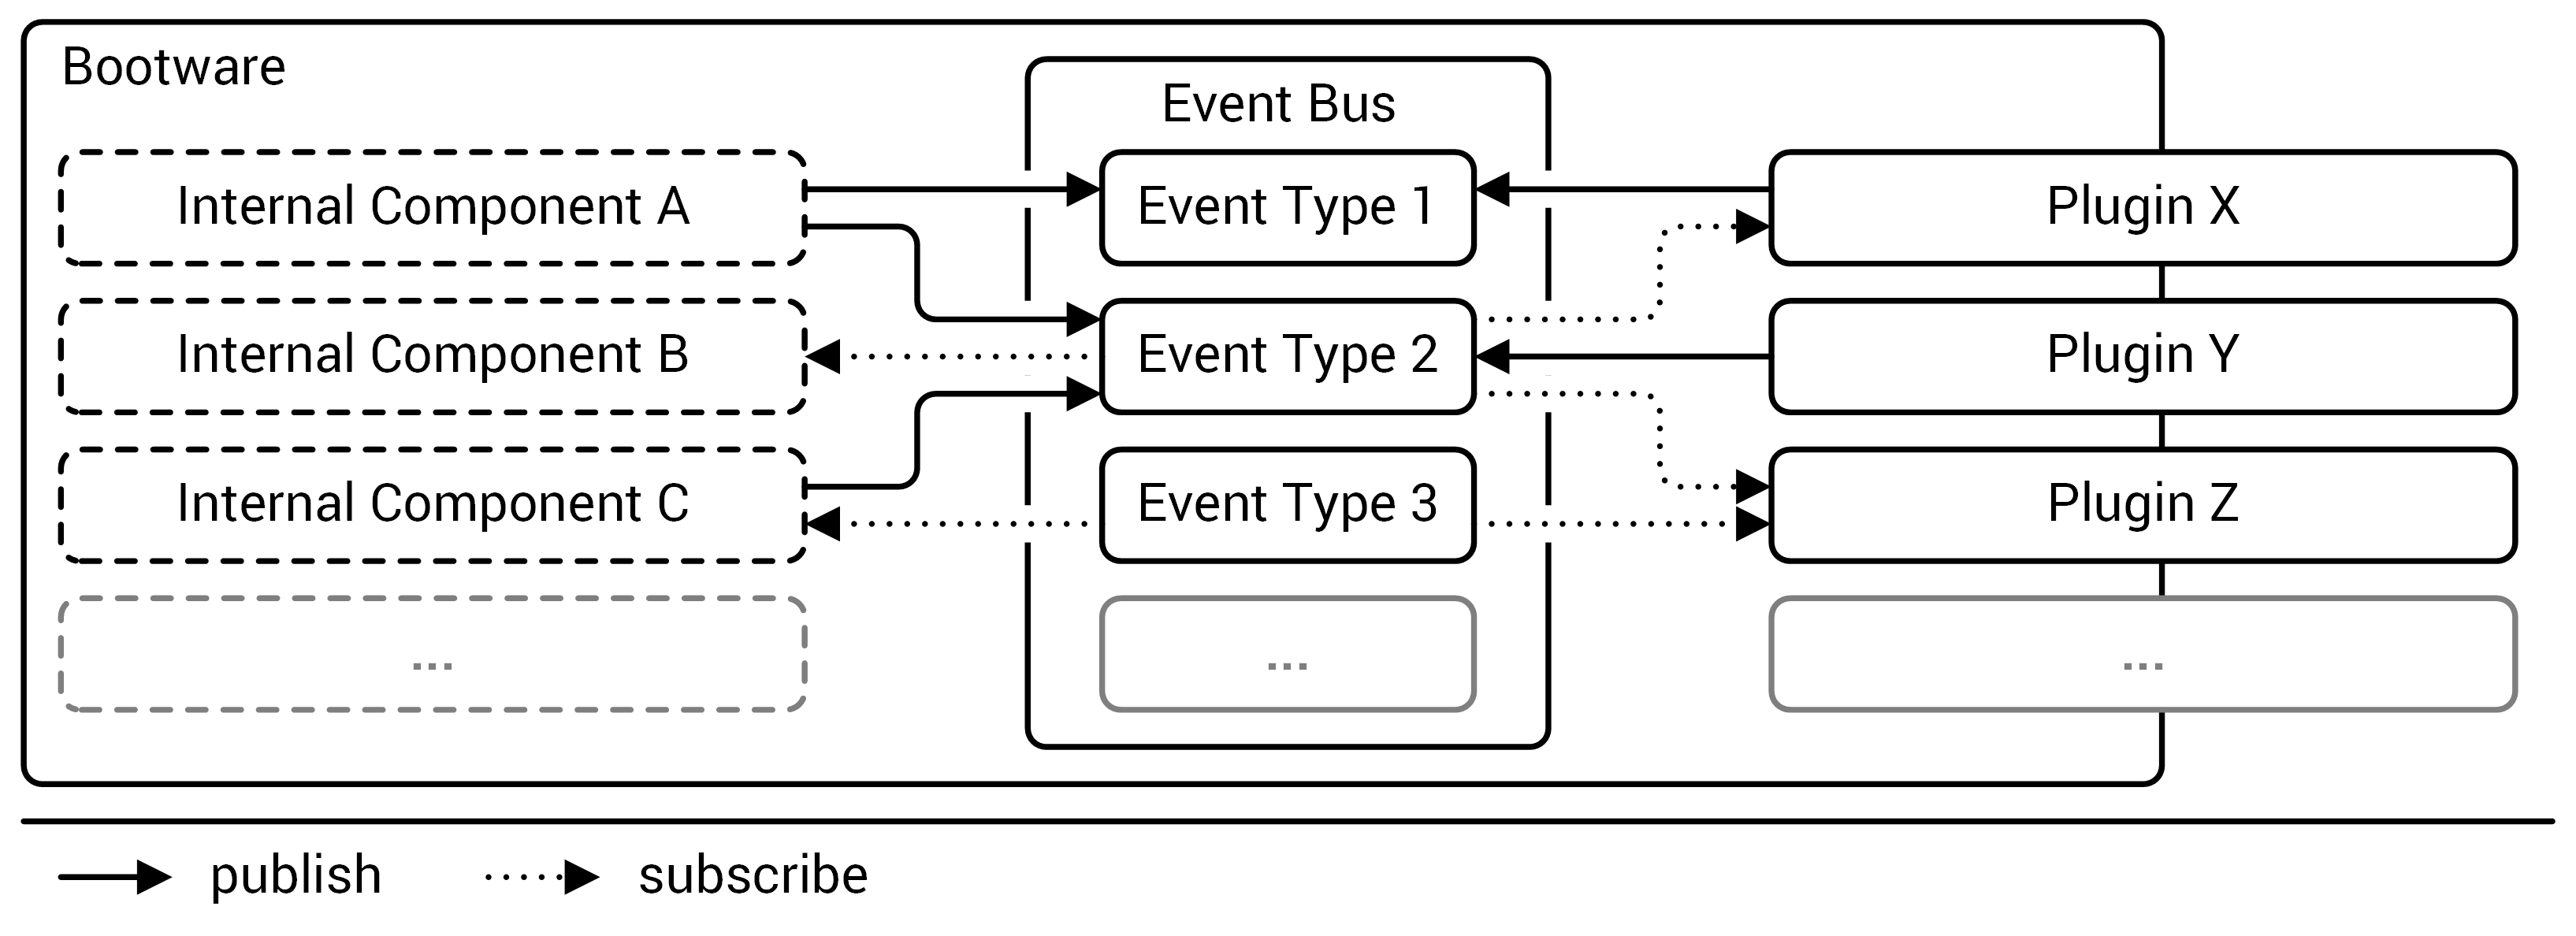
\includegraphics[resolution=600]{design/assets/pubsub}
	\caption{Bootware internal communication with PubSub pattern.}
	\label{image:pubsub}
\end{figure}
